\documentclass[12pt]{article}
\usepackage[margin=1in]{geometry}                % See geometry.pdf to learn the layout options. There are lots.
\geometry{letterpaper}                   % ... or a4paper or a5paper or ... 
%\geometry{landscape}                % Activate for for rotated page geometry
\usepackage[parfill]{parskip}    % Activate to begin paragraphs with an empty line rather than an indent

%%%%%%%%%%%%%%%%%%%%
\newcommand{\hide}[1]{}

\usepackage{natbib}
\usepackage{xcolor}
\usepackage{url}
\usepackage{hyperref}
\usepackage{mathtools}

\hide{
\usepackage{amscd}
\usepackage{amsfonts}
\usepackage{amsmath}
\usepackage{amssymb}
\usepackage{amsthm}
\usepackage{cases}		 
\usepackage{cutwin}
\usepackage{enumerate}
\usepackage{enumitem}
\usepackage{epstopdf}
\usepackage{graphicx}
\usepackage{ifthen}
\usepackage{lipsum}
\usepackage{mathrsfs}	
\usepackage{multimedia}
\usepackage{wrapfig}
}
\bibliographystyle{humanbio}

	 
%\input{/usr/local/LATEX/Lee_newcommands.tex}
\newcommand{\itemlist}[1]{\begin{itemize}#1\end{itemize}}
\newcommand{\enumlist}[1]{\begin{enumerate}#1\end{enumerate}}
\newcommand{\desclist}[1]{\begin{description}#1\end{description}}

\newcommand{\Answer}[1]{\begin{quote}{\color{blue}#1}\end{quote}}
\newcommand{\AND}{\wedge}
\newcommand{\OR}{\vee}
\newcommand{\ra}{\rightarrow}
\newcommand{\lra}{\leftrightarrow}

\title {{\bf Project 1: Distributed Coordination Function} \\
\large{ECE 578: Fundamentals of Computer Networks}}

\author{Lena Voytek and Mitchell Dzurick}
\date{10/22/2019}


\begin{document}
\maketitle{}

\section*{Introduction:}

    This project models four different scenarios where multiple nodes are transmitting packets over an 802.11 network protocol. The first two are based on a network where four nodes are in a single collision domain with two of the nodes transmitting frames in a Poisson-distributed manner. One of them uses generic CSMA/CA {\bf (simulation A1)} while the other also implements virtual carrier sensing {\bf (simulation A2)}. The second set are based on a network where the two nodes are sending to the same receiver while being hidden to one another. Once again, on uses CSMA/CA {\bf (simulation B1)}, while the other implements virtual carrier sensing {\bf (simulation B2)}.
    \par
    The workload was split evenly between the two group members. Most of it was completed as a combined effort between them at the same time, such as the determined code structure and documentation. Lena was responsible of the logic of each simulation and the creation of a general Poisson arrival function. Mitchell was in charge of developing an automated graph creation system and creating a system to build and execute all simulations while outputting to the proper files.
    \par
    Development for the project consisted of the languages C, Make, CMake, Gnuplot, shell scripting, and \LaTeX{}. The actual simulation code was created in C using a set of six files and structs for nodes. Make and CMake were used to automatically compile and run simulations while using the CLion IDE. Gnuplot scripts were developped to automatically create each graph and export them to PNG files. Shell scripting was used to easily run the graph creation scripts. Finally, \LaTeX{} was used to create this document. For more specifics and the actual code, see the project on Github at \\
    \textcolor{blue}{ \href{https://github.com/lvoytek/ECE578/tree/master/DistributedCoordinationFunction}{https://github.com/lvoytek/ECE578/tree/master/DistributedCoordinationFunction}}.
    
    {\bf Simulation A1} - CSMA/CA \\
    {\bf Simulation A2} - CSMA/CA with virtual carrier sensing \\
    {\bf Simulation B1} - CSMA/CA hidden terminals \\
    {\bf Simulation B2} - CSMA/CA hidden terminals with virtual carrier sensing
\clearpage

\section{Throughput T}

    \renewcommand{\labelenumi}{{\bf\alph{enumi})}}
    \begin{enumerate}
        \item { %1A
            {\bf Node A:} Throughput T (Kbps) vs. rate \(\lambda{}\) (frames/sec) for scenarios A and B, and CSMA implementations 1 and 2.
            
            \begin{figure}[!htb]
                \centering
                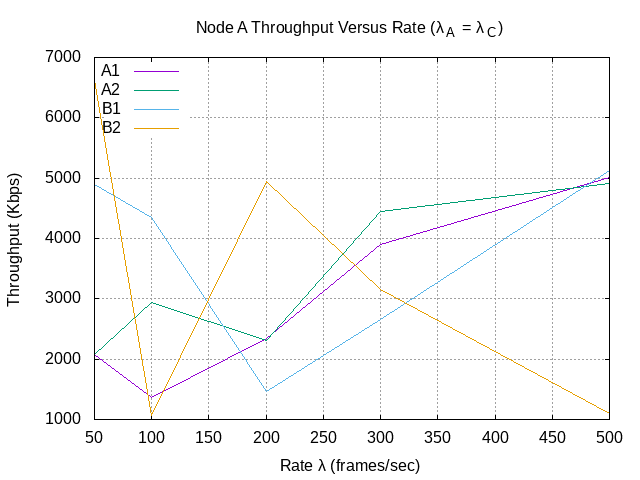
\includegraphics[width=5in]{1A.png}
                \caption{Node A Throughput when \(\lambda{} = \lambda{}_A = \lambda{}_C\) }
                \label{fig:1A}
            \end{figure}
            
            In general, for each Node A using a control \(\lambda{}\) value equal to that of C, the throughput begins with a decrease, followed by a gradual increase as the frame rate increases. The initial decrease is due to the amount of frames coming in overwhelming the network. However, it steadily increases later on as it takes advantage of the larger maximum backoff window delays because of all the collisions.The throughput of simulation B2 takes a different turn though. This is because, with the RTS and hidden terminal, collisions are spread out and it cannot take advantage of the increasing backoff windows.
        }
        
\clearpage

        \item { %1B
            {\bf Node C:} Throughput T (Kbps) vs. rate \(\lambda{}\) (frames/sec) for scenarios A and B, and CSMA implementations 1 and 2.
            
            \begin{figure}[!htb]
                \centering
                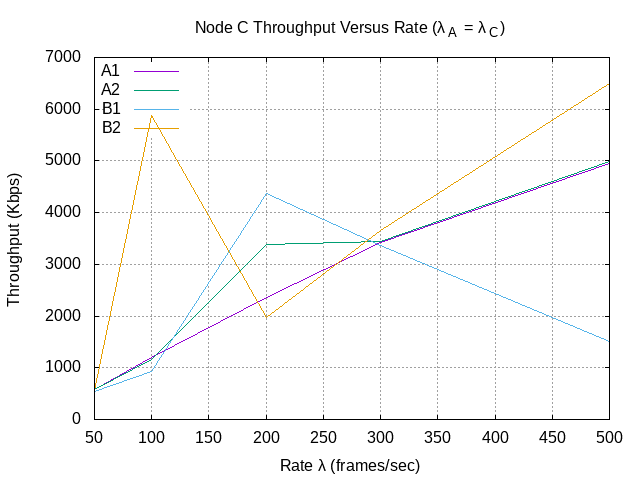
\includegraphics[width=5in]{1B.png}
                \caption{Node C Throughput when \(\lambda{} = \lambda{}_A = \lambda{}_C\) }
                \label{fig:1B}
            \end{figure}

            Node C, unsurprisingly, follows a similar pattern to Node A in throughput when their \(\lambda{}\) values are equivalent. However in this case the throughput skips the slight decrease and follows through with a general increase. This is also the result of increasing backoff times on A combined with the luck of often being the first node to transmit during a certain set of frames. B1 does not quite take advantage of this as it was probably hit with unfortunate frame timing, exacerbated by the fact that the nodes were unable to listen for each other's transmissions.
        }
        
\clearpage
        \item { %1C)
            {\bf Node A:} Throughput T (Kbps) vs. rate \(\lambda{}\) (frames/sec) for scenarios A and B, and CSMA implementations 1 and 2, when \(\lambda{}_A = 2\lambda{}\).
            
            \begin{figure}[!htb]
                \centering
                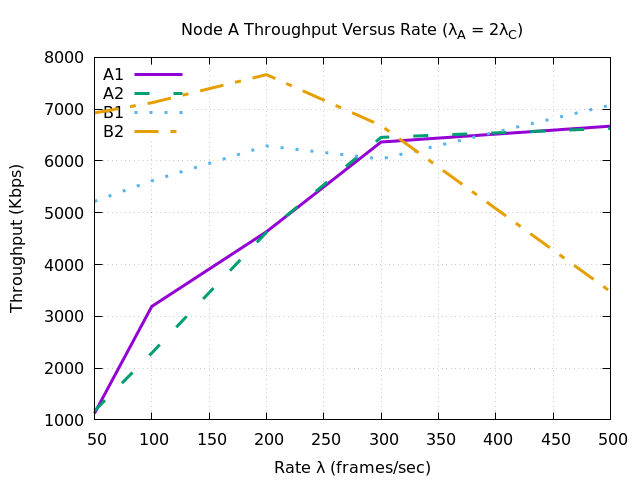
\includegraphics[width=5in]{1C.png}
                \caption{Node A Throughput when \(\lambda{}_A = 2\lambda{}, \lambda{}_C = \lambda{}\) }
                \label{fig:1C}
            \end{figure}
            
            Node A shows a generally increasing Throughput as lambda increases while \(\lambda{}_A = 2\lambda{}\). This makes sense as over time the disparity between the two values increases exponentially. Given the sheer amount of frames arriving at A, its throughput would have to increase to keep up with the greater demand compared to C. As per usual, however, there is an outlier. B2 loses throughput because most of its RTS and CTS frames are colliding with C's, which only gets worse with more frames once the backoff window is saturated.
            
        }
        
\clearpage
        \item { %1D
            {\bf Node C:} Throughput T (Kbps) vs. rate \(\lambda{}\) (frames/sec) for scenarios A and B, and CSMA implementations 1 and 2, when \(\lambda{}_A = 2\lambda{}\).
            
            \begin{figure}[!htb]
                \centering
                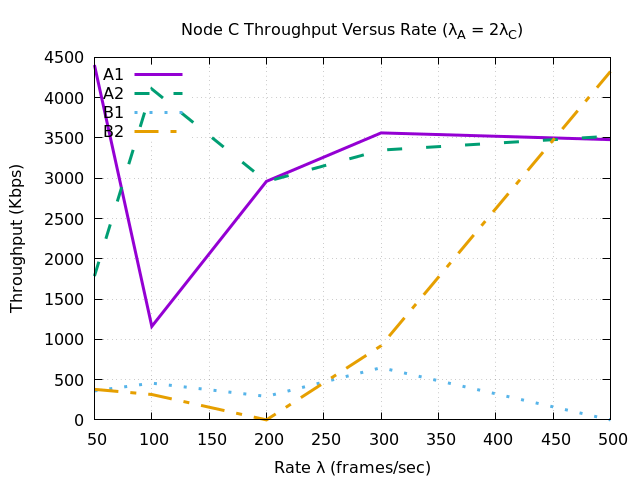
\includegraphics[width=5in]{1D.png}
                \caption{Node C Throughput when \(\lambda{}_A = 2\lambda{}, \lambda{}_C = \lambda{}\) }
                \label{fig:1D}
            \end{figure}

            With the imbalance between \(\lambda{}_A\) and \(\lambda{}_C\), Node C sees results that are all over the place. In general, though, the overall throughput is at around half that of A. This makes sense as Node C has half as many frames arriving. The A simulations are fairly constant as \(\lambda{}\) increases because collision backoff times have maxed out at this point due to Node A overwhelming the channel. B1 also experiences this up until the point where there are so many A frames that none of C's can get through. B2, on the other hand, spikes when it manages to find a sweet spot for RTS collisions that allows it to transmit between A frames.
        }
        
    \end{enumerate}
        
\clearpage        
\section{Collisions N}

    \begin{enumerate}
    
        \item {
            {\bf Node A:} Number of collisions N vs. rate \(\lambda{}\) (frames/sec) for scenarios A and B, and CSMA implementations 1 and 2.
            
            \begin{figure}[!htb]
                \centering
                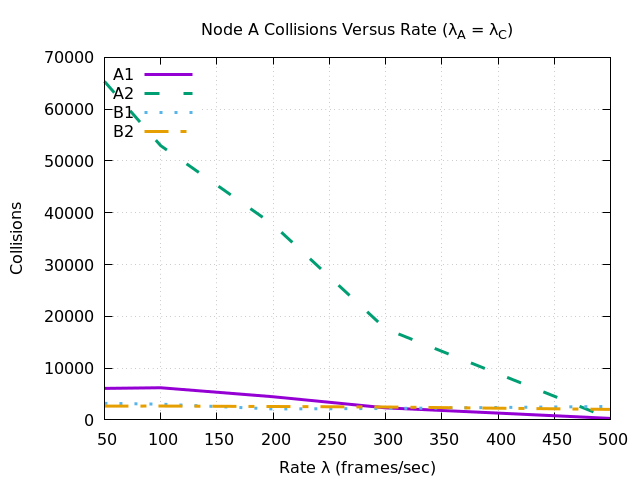
\includegraphics[width=5in]{2A.png}
                \caption{Node A Collisions when \(\lambda{} = \lambda{}_A = \lambda{}_C\) }
                \label{fig:2A}
            \end{figure}

            It may seem counter-intuitive that the collisions of A decrease as the rate of arrival increases. The reason for this is the increasing backoff windows. As more frames come in, a few collisions will push the window to its maximum size, in which fewer new collisions happen. A2 starts off with a particularly high number of collisions because it uses RTS and CTS frames prior to the data. They are much smaller and are more likely to collide often as the countdown collision possibilities increase over a given time interval.  
        }    
    
    
\clearpage  
        \item {
            {\bf Node C:} Number of collisions N vs. rate \(\lambda{}\) (frames/sec) for scenarios A and B, and CSMA implementations 1 and 2.
            
            \begin{figure}[!htb]
                \centering
                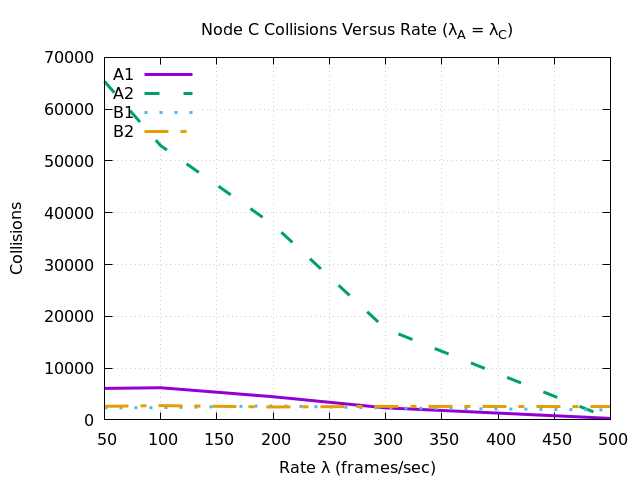
\includegraphics[width=5in]{2B.png}
                \caption{Node C Collisions when \(\lambda{} = \lambda{}_A = \lambda{}_C\) }
                \label{fig:2B}
            \end{figure}

            For collisions happening between nodes on the same collision domain without outside interference, the number of collisions will always be the same. Collisions in this situation can only happen when both nodes' countdowns hit zero at the same time. Hence, for both A simulations, the collisions for node C are the same as node A. As for the B simulations, collisions can happen at any time for each node, but both nodes will take the collision into account. This means that the overall number of collisions for nodes A and C are more or less the same, with slight variation due to the propagation delay. 
        }    
\clearpage  
        \item {
            {\bf Node A:} Number of collisions N vs. rate \(\lambda{}\) (frames/sec) for scenarios A and B, and CSMA implementations 1 and 2, when \(\lambda{}_A = 2\lambda{}\).
            
            \begin{figure}[!htb]
                \centering
                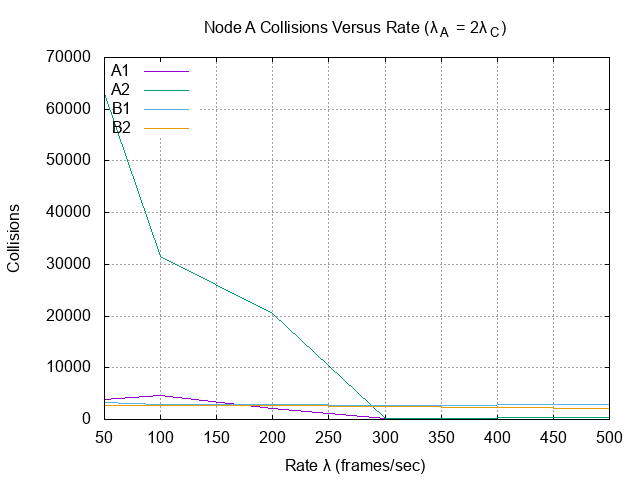
\includegraphics[width=5in]{2C.png}
                \caption{Node A Collisions when \(\lambda{}_A = 2\lambda{}, \lambda{}_C = \lambda{}\) }
                \label{fig:2C}
            \end{figure}

            In the case where \(\lambda{}_A\) is doubled, not much changes in terms of collisions. This is due to the effects of backoff window increases and rate increases cancelling each other out. Once again, A2 starts off very large because of the short delays of determining status with RTS. 
        }        
    
\clearpage  
        \item {
            {\bf Node C:} Number of collisions N vs. rate \(\lambda{}\) (frames/sec) for scenarios A and B, and CSMA implementations 1 and 2, when \(\lambda{}_A = 2\lambda{}\).
            
            \begin{figure}[!htb]
                \centering
                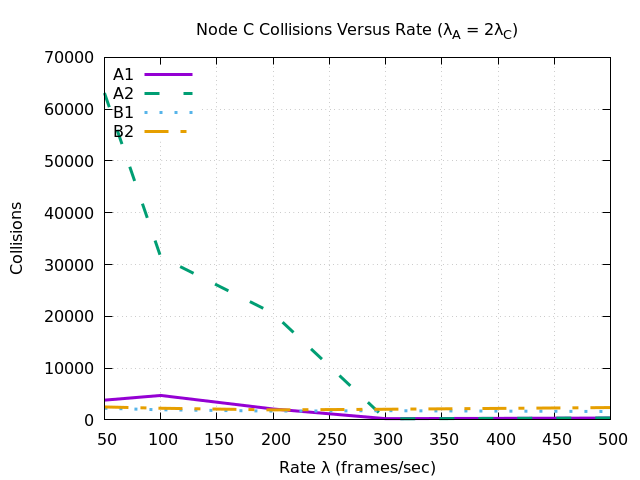
\includegraphics[width=5in]{2D.png}
                \caption{Node C Collisions when \(\lambda{}_A = 2\lambda{}, \lambda{}_C = \lambda{}\) }
                \label{fig:2D}
            \end{figure}

            Like before, the collisions of node C just about match the collisions of node A. The A simulations are exactly the same as the rule of collision on zero countdown has not changed. Meanwhile the B simulations are almost the same with variation from propagation delays.
        }        
    
    
    \end{enumerate}
    
    
\clearpage
    \section{Fairness Index FI}

    \begin{enumerate}
    
        \item {
            Fairness Index FI vs. rate \(\lambda{}\) (frames/sec) for scenarios A and B, and CSMA implementations 1 and 2.
            
            \begin{figure}[!htb]
                \centering
                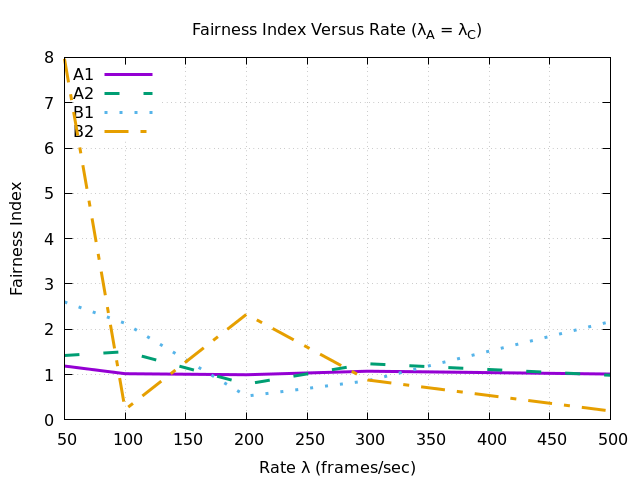
\includegraphics[width=5in]{3A.png}
                \caption{Fairness Index when \(\lambda{} = \lambda{}_A = \lambda{}_C\) }
                \label{fig:3A}
            \end{figure}

            The Fairness Index is the fraction of time that the channel is occupied by a pair A \(\rightarrow\) B over the fraction of time that the channel is occupied by pair C \(\rightarrow\) B or D as a function of \(\lambda\). Therefore, a high Fairness Index indicates that A is transmitting a lot, and the simulation is 'unfair' to pair C \(\rightarrow\) B or D. As shown in Figure 9, the fairness index when \(\lambda{} = \lambda{}_A = \lambda{}_C\) is generally around 1-2 which is a fair result. The major outlier is simulation A2 which a lambda of 50 is very unfair to pair C \(\rightarrow\) B or D, which can be attributed to bad luck with random chance; when A keeps succeeding, C keeps getting blocked out.
        }    
    
    
\clearpage  
        \item {
            Fairness Index FI vs. rate \(\lambda{}\) (frames/sec) for scenarios A and B, and CSMA implementations 1 and 2, when \(\lambda{}_A = 2\lambda{}\).
            
            \begin{figure}[!htb]
                \centering
                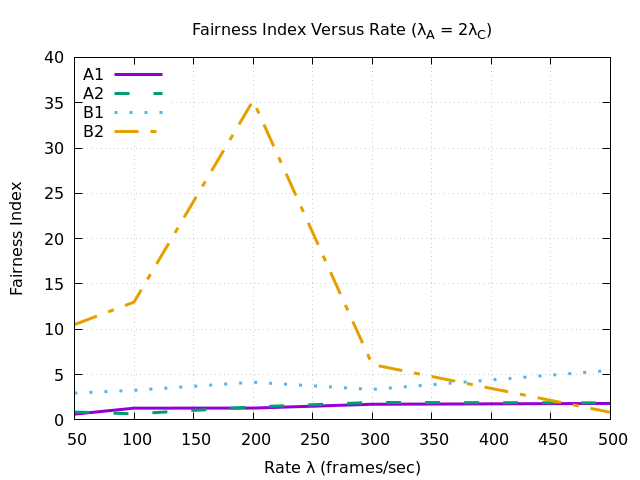
\includegraphics[width=5in]{3B.png}
                \caption{Fairness Index when \(\lambda{}_A = 2\lambda{}, \lambda{}_C = \lambda{}\) }
                \label{fig:3B}
            \end{figure}

            The Fairness Index when \(\lambda{}_A = 2\lambda{}, \lambda{}_C = \lambda{}\) yielded a much different result than when \(\lambda{} = \lambda{}_A = \lambda{}_C\). Figure 9 only goes up to a max Fairness Index of 8 whereas Figure 10 goes up to a max Fairness Index of 35 when \(\lambda\) = 200. The increase in \(\lambda\) for node A decreases the countdown between frames. This decrease in countdown time correlates to node A being favored over node C. Figure 10 shows that, in general, node pair pair A \(\rightarrow\) B is favored much greater when pair A \(\rightarrow\) B has \(\lambda{}_A = 2\lambda{}, \lambda{}_C = \lambda{}\). The simulations most close to a Fairness Index of 1 are simulation A1 (CSMA/CA) and B1 (CSMA/CA w/ hidden terminals), which show that adding virtual carrier sensing only hurts the throughput of pair C \(\rightarrow\) B or D.
        }    
    \end{enumerate}
\end{document}  
%%%%%%%%%%%%%%%%%%%%%%%%%%%%%%%%%%%%%%%%%%%%%%